\begin{table}[t]
\begin{minipage}{.49\linewidth}
    \begin{minipage}{\textwidth}
        \centering
        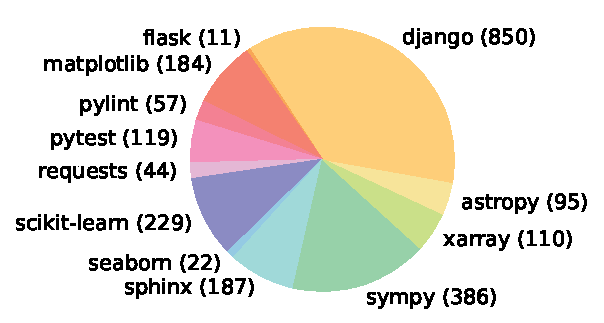
\includegraphics[width=\textwidth]{figures/assets/task-distribution.pdf}
        \captionof{figure}{
        Distribution of \benchmark{} tasks (in parenthesis) across 12 open source GitHub repositories that each contains the source code for a popular, widely downloaded PyPI package.
        }
        \label{fig:task-distribution}
    \end{minipage}
\end{minipage}
\hfill
\begin{minipage}{.48\linewidth}
    \begin{minipage}{\textwidth}
        \centering
        \caption{
        Average and maximum numbers characterizing different attributes of a \benchmark{} task instance.
        Statistics are micro-averages calculated without grouping by repository.
        }
        \resizebox{\textwidth}{!}{
        \small
        \begin{tabular}{llrr}
        \toprule
            & & Mean & Max \\
        \midrule
            Issue Text & Length (Words) & 195.1 & 4477 \\
            \midrule
            \multirow{2}{*}{Codebase} & \# Files (non-test) & 3,010 & 5,890 \\
                                      & \# Lines (non-test) & 438K  & 886K \\
            \midrule
            \multirow{3}{*}{Gold Patch} & \# Lines edited & 32.8 & 5888 \\
                                        & \# Files edited & 1.7 & 31 \\
                                        & \# Func. edited & 3 & 36 \\
            \midrule
            \multirow{2}{*}{Tests} & \# Fail to Pass & 9.1 & 1633 \\
                                   & \# Total & 120.8 & 9459 \\
        \bottomrule
        \end{tabular}
        }
        \label{table:dataset-stats}
    \end{minipage}
\end{minipage}
\vspace{-0.5em}
\end{table}
